% \chapter[Elementos do Texto]{Elementos do Texto}

% \section{Corpo do Texto}

% O estilo de redação deve atentar a boa prática da linguagem técnica. Para a 
% terminologia metrological usar o Vocabulário Internacional de Termos 
% Fundamentais e Gerais de Metrologia \cite{inmetro2003}  (Instituto Nacional de Metrologia, 
% 2003).

% Grandezas dimensionais devem ser apresentadas em unidades consistentes com 
% o Sistema Internacional de Unidades  (SI). Outras unidades podem ser usadas 
% como unidades secundárias entre parenteses se necessário. Exceções são 
% relacionadas a unidades não-SI usadas como identificadores comerciais como 
% pro exemplo \lq\lq disquete de  3$\nicefrac{1}{2}$ polegadas\rq\rq. 

% Na apresentação de números ao longo do texto usar virgula para separar a 
% parte decimal de um número. Resultados experimentais devem ser apresentados 
% com sua respectiva incerteza de medição.

% \section{Títulos de capítulos e seções}

% Recomendações de formatação de seções 

% \begin{description}

% 	\item \textbf{1 SEÇÃO PRIMÁRIA - MAIÚSCULAS; NEGRITO; TAMANHO 12;}

% 	\item 1.1 SEÇÃO SECUNDÁRIA – MAIÚSCULAS; NORMAL; TAMANHO 12; 

% 	\item \textbf{1.1.1 Seção terciária - Minúsculas, com exceção da 
% 	primeira letra; negrito; tamanho 12;}

% 	\item 1.1.1.1 Seção quaternária - Minúsculas, com exceção da primeira 
% 	letra; normal tamanho 12; 

%  	\item \textit{1.1.1.1.1 Seção quinária - Minúsculas, com exceção da 
% 	primeira letra; itálico; tamanho 12.}

% \end{description}

% \section{Notas de rodapé}

% Notas eventualmente necessárias devem ser numeradas de forma seqüencial ao 
% longo do texto no formato 1, 2, 3... sendo posicionadas no rodapé de cada 
% página na qual a nota é utilizada.\footnote{Como, por exemplo, esta nota}

% \section{Equações}

% Equações matemáticas devem ser numeradas seqüencialmente e alinhadas a 
% esquerda com recuo de 0,6 cm. Usar numerais arábicos entre parênteses, 
% alinhado a direita, no formato Times New Roman de 9 pts. para numerara as 
% equações como mostrado na Eq. (\ref{eqn01}).

% Referências a equações no corpo do texto devem ser feitas como \lq\lq Eq. 
% (\ref{eqn01})\rq\rq\ quando no meio de uma frase ou como \lq\lq Equação 
% (\ref{eqn01})\rq\rq\ quando no inicio de uma sentença. Um espaçamento de 11 
% pontos deve ser deixado acima, abaixo e entre equações subseqüentes. Para uma 
% apresentação compacta das equações deve-se usar os símbolos e expressões 
% matemáticos mais adequados e parênteses para evitar ambigüidades em 
% denominadores. Os símbolos usados nas equações citados no texto devem 
% apresentar exatamente a mesma formatação usada nas equações.
% \begin{equation}
% \label{eqn01}
% 	\frac{d\mathbf{C}}{dw} = \frac{du}{dw}\cdot \mathbf{F}_u + 
% 		\frac{dv}{dw}\cdot \mathbf{F}_v 
% \end{equation}

% O significado de todos os símbolos mostrados nas equações deve ser apresentado 
% na lista de símbolos no inicio do trabalho, embora, em certas circunstancias o 
% autor possa para maior clareza descrever o significado de certos símbolos no 
% corpo do texto, logo após a equação.

% \section{Figuras e Gráficos}

% As figuras devem ser centradas entre margens e identificadas por uma legenda 
% alinhada a esquerda com recuo especial de deslocamento de 1,8 cm, com mostrado 
% na Fig. (\ref{fig01}). O tamanho das fontes empregadas nos rótulos e anotações 
% usadas nas figuras deve ser compatível com o usado no corpo do texto. Rótulos e 
% anotações devem estar em português, com todas as grandezas mostradas em 
% unidades do SI (Sistema Internacional de unidades).

% Todas as figuras, gráficos e fotografias devem ser numeradas e referidas no 
% corpo do texto adotando uma numeração seqüencial de identificação. As figuras e 
% gráficos devem ser claras e com qualidade adequada para eventual reprodução 
% posterior tanto em cores quanto em preto-e-branco.

% As abscissas e ordenadas de todos os gráficos devem ser rotuladas com seus 
% respectivos títulos em português seguida da unidade no SI que caracteriza a 
% grandes entre colchetes. 

% A referência explícita no texto à uma figura deve ser feita como 
% \lq\lq Fig. (\ref{fig01})\rq\rq\ quando no meio de uma frase ou como 
% \lq\lq Figura (\ref{fig01})\rq\rq\ quando no início da mesma. Referencias 
% implícitas a uma dada figura devem ser feitas entre parênteses como 
% (Fig. \ref{fig01}). Para referências a mais de uma figura as mesmas regras 
% devem ser aplicadas usando-se o plural adequadamente. Exemplos:

% \begin{itemize}
% 	\item \lq\lq Após os ensaios experimentais, foram obtidos os resultados 
% 	mostrados na Fig. (\ref{fig01}), que ...\rq\rq
% 	\item \lq\lq A Figura (\ref{fig01}) apresenta os resultados obtidos, onde 
% 	pode-se observar que ...\rq\rq
% 	\item \lq\lq As Figuras (1) a (3) apresentam os resultados obtidos, 
% 	...\rq\rq
% 	\item \lq\lq Verificou-se uma forte dependência entre as variáveis citadas 
% 	(Fig. \ref{fig01}), comprovando ...\rq\rq
% \end{itemize}

% Cada figura deve ser posicionada o mais próxima possível da primeira citação 
% feita à mesma no texto, imediatamente após o parágrafo no qual é feita tal 
% citação, se possível, na mesma página.
% \begin{figure}[h]
% 	\centering
% 	\label{fig01}
% 		\includegraphics[keepaspectratio=true,scale=0.3]{figuras/fig01.eps}
% 	\caption{Wavelets correlation coefficients}
% \end{figure}

% \section{Tabela}

% As tabelas devem estar centradas entre margens e identificadas por uma legenda 
% alinhada a esquerda, com recuo especial de deslocamento de 1,8 cm, posicionada 
% acima da tabela com mostrado nas Tabs. (\ref{tab01}) e (2), a título de 
% exemplo. O tamanho das fontes empregadas nos rótulos e anotações usadas nas 
% tabelas deve ser compatível com o usado no corpo do texto. Rótulos e anotações 
% devem estar em português. Um espaçamento de 11 pts deve ser deixado entre a 
% legenda e a tabela, bem como após a tabela. 

% As grandezas dimensionais mostradas em cada tabela devem apresentar unidades 
% consistentes com o SI. As unidades de cada variável devem ser mostradas apenas 
% na primeira linha e/ou coluna da tabela, entre colchetes 

% A referência explícita no texto à uma dada tabela deve ser feita como 
% \lq\lq Tab. (\ref{tab01})\rq\rq\ quando no meio de uma frase ou como 
% \lq\lq Tabela (\ref{tab01})\rq\rq\ quando no início da mesma. Referências 
% implícitas a uma dada tabela devem ser feitas entre parênteses como 
% \lq\lq (Tab. \ref{tab01}). Para referências a mais de uma tabela as mesmas 
% regras devem ser aplicadas usando-se o plural adequadamente. Exemplos:
% \begin{itemize}
% 	\item \lq\lq Após os ensaios experimentais, foram obtidos os resultados 
% 	mostrados na Tab. (\ref{tab01}), que ...\rq\rq
% 	\item \lq\lq A Tabela (\ref{tab01}) apresenta os resultados obtidos, onde 
% 	pode-se observar que ...\rq\rq
% 	\item As Tabelas (1) a (3) apresentam os resultados obtidos, ...\rq\rq
% 	\item Verificou-se uma forte dependência entre as variáveis citadas 
% 	(Tab. \ref{tab01}), comprovando ...\rq\rq
% \end{itemize}

% Cada tabela deve ser posicionada o mais próxima possível da primeira citação 
% feita à mesma no texto, imediatamente após o parágrafo no qual é feita a 
% citação, se possível, na mesma página.

% \begin{table}[h]
% 	\centering
% 	\label{tab01}
	
% 	\begin{tabular}{ccc}
% 		\toprule
% 		\textbf{Processing type} & \textbf{Property 1} (\%) & 
% 		\textbf{Property 2} $[\mu m]$ \\
% 		\midrule
% 		Process 1 & 40.0 & 22.7 \\
% 		Process 2 & 48.4 & 13.9 \\
% 		Process 3 & 39.0 & 22.5 \\
% 		Process 4 & 45.3 & 28.5 \\
% 		\bottomrule
% 	\end{tabular}

% 	\caption{Propriedades obtidades após processamento}
% \end{table}

% \section{Citação de Referências}

% Referencias a outros trabalhos tais como artigos, teses, relatórios, etc. devem 
% ser feitas no corpo do texto devem estar de acordo com a norma corrente ABNT 
% NBR 6023:2002 (ABNT, 2000), esta ultima baseada nas normas ISO 690:1987:
% \begin{itemize}
% 	\item \lq\lq \cite{bordalo1989}, mostraram que...\rq\rq

% 	\item \lq\lq Resultados disponíveis em \cite{coimbra1978}, \cite{clark1986} 
% 	e \cite{sparrow1980}, mostram que...\rq\rq
% \end{itemize}

% Para referências a trabalhos com até dois autores, deve-se citar o nome de 
% ambos os autores, por exemplo: \lq\lq \cite{soviero1997}, mostraram 
% que...\rq\rq

\part{Desenvolvimento}

\chapter{Fundamentação Teórica}

Neste capitulo será apresentado os conceitos e referências utilizadas para a construção deste trabalho. Alguns algoritmos apontados neste trabalho foram publicados com objetivos distintos dos utilizados atualmente ou eram unicamente teóricos devido ao contexto da época onde a computação e os avanços tecnológicos eram motivos de limitação para uma aplicação real destes algoritmos. Dos que foram designados para objetivos distintos de aproximação de \textit{strings}, é notável quantos deles surgiram da área de biologia, no intuito de semelhanças de especies ou proximidades genéticas.

Para as contribuições para código aberto, a filosofia apresentada pela comunidade é a de trabalho em conjunto, com  produção em massa de diversos pontos de vista distintos, a fim de oferecer a melhor funcionalidade e manter um alto grau de confiabilidade em segurança.

\input editaveis/conteudo/gerenciadores
\input editaveis/conteudo/apt
\input editaveis/conteudo/stringmatching
\chapter{Metodologia e Procedimentos}

Neste capitulo será apresentada a forma como os experimentos serão realizados, assim como o ambiente  utilizado para obter estes resultados. Por se tratar de uma contribuição dividida em etapas cíclicas, elas serão apresentadas divididas em sessões.

\input editaveis/conteudo/metodo
\input editaveis/conteudo/contribuindo

\part{\nmu Resultados}
\label{part:resultados}

\chapter{Coleta de Dados} % (fold)
\label{cha:coleta_de_dados}

\section{Tempo} % (fold)
\label{sec:tempo}

A coleta de tempo de performance de um software é árdua. A estimativa de tempo depende das otimizações que o compilador pode vir a fazer para a arquitetura, memoria disponível, aplicativos rodando em concorrência, temperatura do hardware, etc. No intuito de simplificar o processo de estimativa de tempo, foi utilizado a mediana de uma serie de chamadas da aplicação. Segundo \citeonline{dolan2002benchmarking}, esta solução pode vir ser a melhor para um ponto geral de $25\%$ das possíveis alternativas de coletas de dados. Assim sendo, o \autoref{scriptods} foi uma solução desenvolvida que permitisse deixar a maquina com tempo dedicado para a aquisição de dados.

Para o funcionamento do \textit{script}, as variáveis {\code MAX} e {\code \_MAX\_THREADS} devem ser definidas com a quantidade de dados que se deseja coletar e a quantidade máxima de \textit{threads} que devem ser levantadas para a chamada do processo respectivamente. Usar uma quantidade superior a quantidade de \textit{cores}  da maquina pode produzir valores com baixa confiabilidade, visto a concorrência gerada pelas \textit{threads}. Como parâmetros, foram escolhidos $150$ dados com $7$ \textit{threads}, possibilitando haver ao menos $1$ \textit{core} livre. Para maior dinamismo da coleta dos dados, o \textit{script} é responsável por realizar a troca das \textit{branchs} onde estão localizadas as possíveis soluções e a compilação e concentração dos dados em uma planilha do \textit{LibreOffice Calc}. Assim, os algoritmos nunca são executados em concorrência, porém os dados serão coletado sob a demanda da $CPU$ em que o \textit{script} é executado.

No intuito de coletar o tempo pontual do algoritmo, o \autoref{libtime} foi desenvolvido a fim de ser usado como cronometro. O algoritmo desenvolvido com o auxilio da biblioteca {\code Chrono}\footnote{A biblioteca é disponibilizada no {\code C++11} sob o \textit{namespace} {\code std::crono::}.} permite a captura do intervalo de tempo com ate $9$ casas decimais de segundos (nanosegundos), todavia foi utilizado a precisão de microssegundos apenas, visto que o intervalo de nanosegundos não iria gerar alto impacto na diferença dos valores. Os métodos {\code begin} e {\code end} da classe são utilizados para pontuar os intervalos onde o tempo deve ser contado. O resultado da contagem pode ser obtido com o retorno do método {\code end} ou com a chamada do {\code currenttime}, dedicado apenas para o retorno deste valor.

\section{Memória}

Para a coleta de memória, foi utilizado o {\code Valgrind} com o auxilio da ferramenta {\code Massif}. Devido a haver uma criação de \textit{hash} de forma  algébrica e o método de \textit{KMP} faz uso de um autômato finito determinístico, a previa repetição das buscas com apenas $10$ ciclos confirmavam a suspeita de não haver a variação do gasto de memória para a repetição da ação.

Para a execução da aplicação com o suporte do {\code Valgrind} para analise do uso de memória, foi utilizado o seguinte comando:

\begin{lstlisting}[language=Bash,label=valgrind_call, numbers=none]
   $ valgrind --tool=massif  ./apt search pacote [--regex]
\end{lstlisting}
% section tempo (end)
% chapter coleta_de_dados (end)


\chapter{Analise de Resultados} % (fold)
\label{cha:analise_de_resultados}

\section{Algorítimos de \textit{string matching} exatos} % (fold)
\label{sec:algor_timos_de_string_matching_exatos}

Para a busca com algorítimos de \textit{string matching} exatos, foram considerado três métodos distintos:

\begin{description}
	\item[Expressão Regular:] Método atual de como a verificação é realizada atualmente. Foi previamente comentado na sessão de \nameref{sec:algoritimos_de_textit}.
	\item[Knuth-Morris-Pratt:] Método que faz de uso do conceito de autômatos de estados para agilizar a busca. Previamente apresentado na sessão \nameref{ssub:knuth_morris_pratt_}.
	\item[Rabin-Karpin:]  Método que faz de uso de \textit{hash}. Foi previamente comentado na sessão \nameref{ssub:rabin_karp}.
\end{description}

Após a coleta de $150$ chamadas de cada pacote usando os algorítimos apontados acima, a \autoref{ssub:rabin_karp} foi criada contendo a mediana dos tempos de execução de cada método para os pacotes selecionados.

\begin{figure}[htbp]
  \centering
  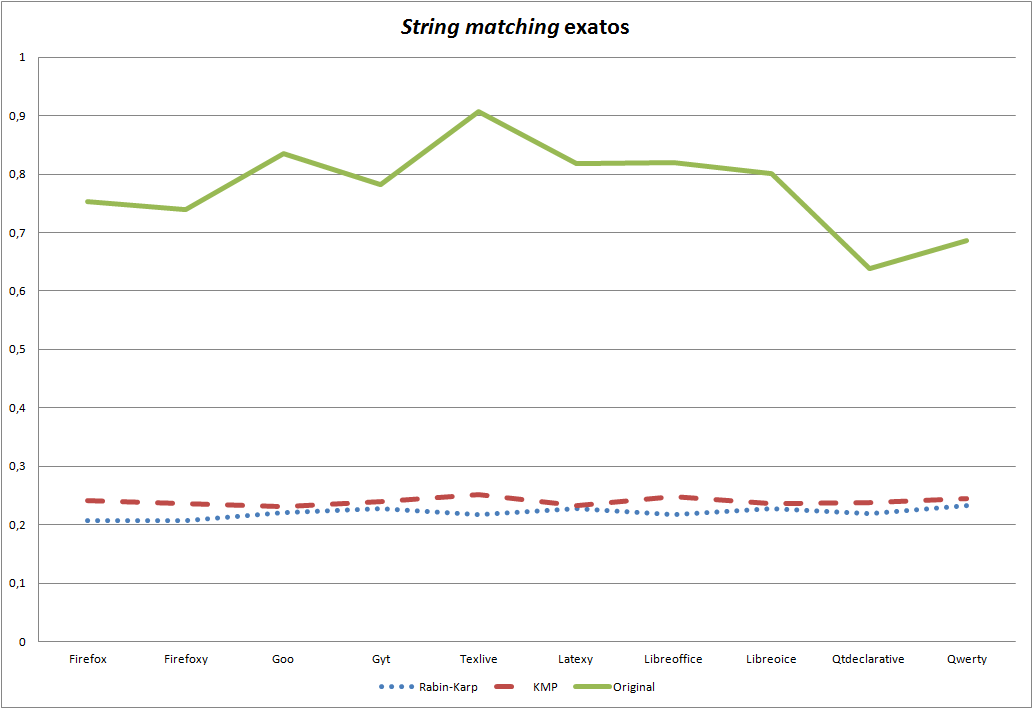
\includegraphics[width=0.95\textwidth]{figuras/tempo-rk_kmp_std}
  \caption{Estimativa de tempo para pacotes usando algorítimos de busca exata}
  \label{tempo_rk_kmp_std}
\end{figure}

Como podemos observar, tanto o \textit{Rabin-Karpin} quanto o \textit{KMP} tiveram um rendimento de cerca de $\frac{1}{3}$ do tempo gasto atualmente com o uso de expressões regulares, sendo no tempo geral, o método de \textit{Rabin-Karpin} possui um desempenho ligeiramente melhor.


\begin{figure}[htbp]
  \centering
  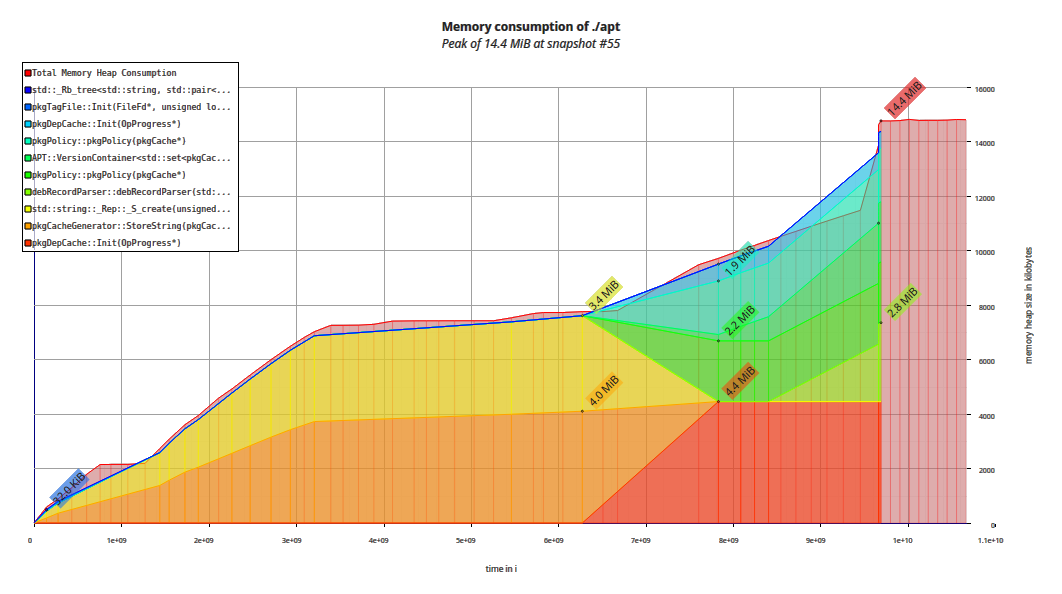
\includegraphics[width=0.95\textwidth]{figuras/memory_rk.png}
  \caption{Apontamento de uso de memória com uso do método de \textit{Rabin-Karpin}}
  \label{memory_rk}
\end{figure}

O consumo total de memória para ambos os métodos, \textit{Rabin-Karpin} na \autoref{memory_rk} e expressões regulares na \autoref{memory_std},  apresentaram resultados similares, porém o método de \textit{Rabin-Karpin} faz um uso de memória mais pontual, alcançando o pico de consumo ao final do processo, quando esta prestes a liberar os recursos. Já o método de expressões regulares apresenta um consumo mais linear de memória. 


\begin{figure}[htbp]
  \centering
  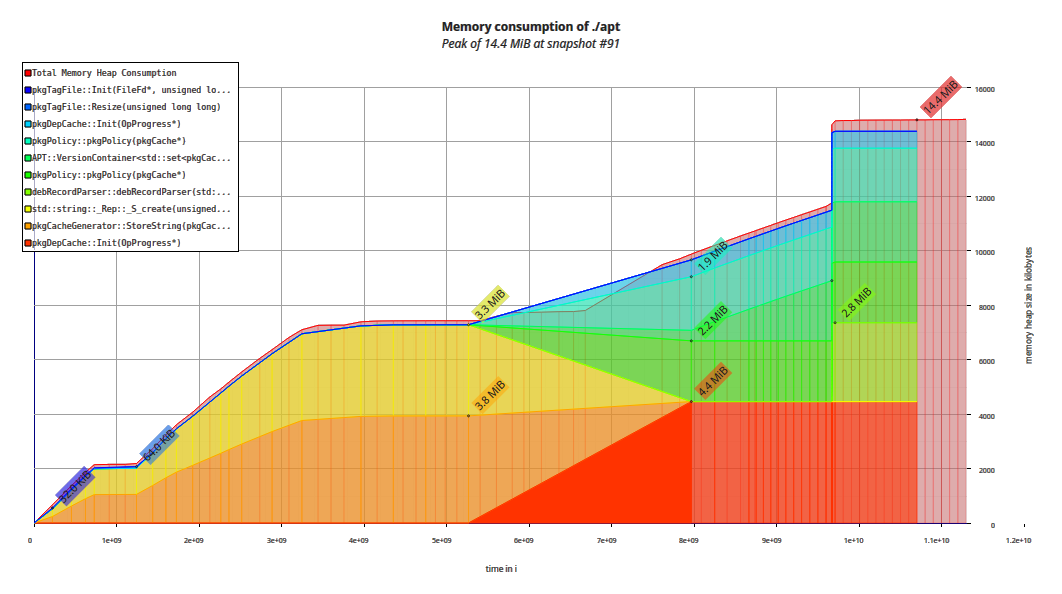
\includegraphics[width=0.95\textwidth]{figuras/memory_regex.png}
  \caption{Apontamento de uso de memória com uso de expressões regulares}
  \label{memory_std}
\end{figure}

Um gasto mais prologado de memória vem a ser prejudicial para sistemas em que diversos processos possam estar sendo executados em conjunto, todavia o grau de consumo é muito baixo para o posicionamento de que o consumo por um período mais extenso venha a ser prejudicial, visto que para um sistema com $2GB$ de memória RAM, $15MB$ seria um valor irrisório de menos de $1\%$ do total de recurso disponível.
% chapter analise_de_resultados (end)

